\input{head.inc}
  
% Präambelbefehle für die Präsentation
\title[TET: Elektromagnetische Wellen III - Harmonische Ebene Wellen]{Elektromagnetische Wellen III - Harmonische Ebene Wellen}

\begin{document}
% 
% Frontmatter 
% 
%%%%%%%%%%%%%%%%%%%%%%%%%%%%%%%%%%%%%%%%%%%%%%%%%%%%%%%%%%%%%%%%%%%%%%%%%%%%%%%%%%%%%%%%%%%%%%%%%%%%%%%%%%%%%%%%%%%%%%%%%%%%% 

%% inserts the title page and the table of contents
\maketitle

% 
% Content 
% 
%%%%%%%%%%%%%%%%%%%%%%%%%%%%%%%%%%%%%%%%%%%%%%%%%%%%%%%%%%%%%%%%%%%%%%%%%%%%%%%%%%%%%%%%%%%%%%%%%%%%%%%%%%%%%%%%%%%%%%%%%%%%% 
\section{Elektromagnetische Wellen III - Harmonische Ebene Wellen}

\begin{frame}
  \frametitle{Ausgangspunkt}
  \begin{itemize}[<+->]
  \item \alert{Homogene} Wellengleichung \(\square\Psi = \left(\laplace - \varepsilon\mu\dfrac{\d^2}{\d t^2} \right)\Psi =0\)
  \item \(\Psi\): eine Komponente der Felder bzw. Vektorpotentials oder das Skalarpotential
  \item \alert{Lorenzeichung}: \(\divergenz\magvekpot[v] +\varepsilon\mu \frac{\d \elpotential}{\d t}=0 \)
  \item \alert{Ebene Wellen} sind Lösungen der Gleichung \(\to\) betrachte nur die \alert{hinlaufende} Lösung für einen Wert von \(\omega\)
    \begin{equation*}
      \Psi(\ortsvektor[v], t) = \Psi(\varphi_-(\ortsvektor[v], t)) = \Psi(\omega t - \wellenzahl[v]\cdot\ortsvektor[v])
    \end{equation*}
  \item Wir wählen nun eine spezielle Phasenfunktion \(\varphi\), so dass \(\Psi\) einer Funktion mit \alert{harmonischer Zeitabhängigkeit} entspricht:
    \begin{equation*}
      \boxed{\underline{\Psi}(\ortsvektor[v], t) = \underline{\Psi}_0 \euler^{\komplex(\omega t -\wellenzahl[v] \cdot \ortsvektor[v])} }\pointspace ; \pointspace \Psi(\ortsvektor[v], t) = \real{\underline{\Psi}(\ortsvektor[v], t)}
      \end{equation*}
  \end{itemize}
\end{frame}


\begin{frame}
  \frametitle{Wellenlänge und Frequenz harm. ebener Wellen}
    \begin{equation*}
      \boxed{\underline{\Psi}(\ortsvektor[v], t) = \underline{\Psi}_0 \euler^{\komplex(\omega t -\wellenzahl[v] \cdot \ortsvektor[v])} }\pointspace ; \pointspace \Psi(\ortsvektor[v], t) = \real{\underline{\Psi}(\ortsvektor[v], t)}
      \end{equation*}
  \begin{itemize}[<+->]
  \item \alert{Fester Zeitpunkt}: Flächen gleicher Werte (= gleicher Phase) haben einen Abstand
    \begin{align*}
&&\Delta\ortsvektor[v]\cdot\wellenzahl[v] &= 2\pi n &&n\in\IZ\\
\ergo &n = 1 : &\Delta\ortsvektor_\Vert \cdot \wellenzahl &= 2\pi &\ergo &\boxed{\Delta \ortsvektor_\Vert = \frac{2\pi}{\wellenzahl} =\lambda}\quad \text{\alert{Wellenlänge}}\\
&& \wellenzahl = \frac{2\pi}{\lambda}&= \frac{\omega}{\geschw_{\mathrm{p}}} &\ergo&\boxed{\geschw_{\mathrm{p}}=\frac{\omega}{2\pi}\cdot \lambda}\pointspace = \geschw_{c} \underset{\substack{\varepsilon = \varepsilon_0 \\ \mu = \mu_0}}{=} \lichtgeschw
\end{align*}
\item \alert{Fester Ort}: Flächen gleicher Werte wiederholen sich nach einer Zeit
\begin{align*}
&&\Delta t \omega &= 2\pi  n && n\in \IZ\\
& n=1: &\Delta t = T &= \nicefrac{2\pi}{\omega} = \nicefrac{1}{f}&&
f:\text{ \alert{Frequenz}}\\
&&&&&\omega:\text{ \alert{Kreisfrequenz}}\\
&&&&&T:\text{ \alert{Periode}}\\
&\ergo & \boxed{\geschw_{\mathrm{p}}= f \cdot \lambda}&= \geschw_{c}\underset{\substack{\varepsilon = \varepsilon_0 \\ \mu = \mu_0}}{=} \lichtgeschw
\end{align*}
  \end{itemize}
\end{frame}

\begin{frame}
  \frametitle{Lösung für die Felder \(\efeld[v]\) und \(\tetB[v]\)}
  \begin{itemize}[<+->]
  \item Ausgangspunkt: \alert{Ebene} Welle mit \alert{harmonischer} Zeitabhängigkeit (Kreisfrequenz \(\omega\)), die in \alert{positiver} \(\wellenzahl[v]\)-Richtung propagiert (\enquote{-}-Lösung)
  \item Wir nehmen zunächst an, dass \(\efeld[v]\) und \(\tetB[v]\) unterschiedliche Kreisfrequenzen und Wellenvektoren haben könnten:
\begin{align*}
\efeld[uv] &= \efeld[uv]_0 \euler^{\komplex(\omega t - \wellenzahl[v]\cdot\ortsvektor[v])}& \tetB[uv] &= \tetB[uv]_0 \euler^{\komplex(\omega ' t - \wellenzahl[v] \ensuremath{'}\cdot\ortsvektor[v])}
\end{align*}
\(\rightarrow\) unterschiedliche Frequenzen und Wellenvektoren \(\omega, \omega', \wellenzahl[v],\wellenzahl[v]'\)
\item Einsetzen in Maxwell-Gleichungen:
\begin{align*}
&\rotation \efeld[uv] = -\frac{\d \tetB[uv]}{\d t}= -\komplex \omega ' \tetB[uv] \text{ andererseits } \rotation \efeld[uv] = -\komplex\left( \wellenzahl[v] \times \efeld[uv]\right)\\
\Rightarrow & -\komplex\left( \wellenzahl[v] \times \efeld[uv]_0 \right) \euler^{\komplex\left(\omega t - \wellenzahl[v]\cdot\ortsvektor[v]\right)} \istgleich -\komplex \omega' \tetB[uv]_0 \euler^{\komplex \left(\omega' t -\wellenzahl[v]'\cdot\ortsvektor[v]\right)}
\end{align*}
\item Soll für alle \(t\) und alle \(\ortsvektor[v]\) gelten:
\begin{align*}
  \ergo & \left. \begin{array}{l}
\omega = \omega'\pointspacek \pointspace \wellenzahl[v] = \wellenzahl[v]'\\
\wellenzahl[v]\times\efeld[uv]_0 = \omega\tetB[uv]_0
                 \end{array}
\right\rbrace \tetB[uv]_0 = \frac{1}{\omega} \wellenzahl[v] \times\efeld[uv]_0 \to \boxed{\tetB[uv] = \frac{1}{\omega} \wellenzahl[v] \times\efeld[uv]}\\
\end{align*}
  \end{itemize}
\end{frame}


\begin{frame}
  \frametitle{Lösung für die Felder \(\efeld[v]\) und \(\tetB[v]\) (\dots)}
 \begin{itemize}[<+->]
\item \( \tetB[uv] = \dfrac{1}{\omega} \wellenzahl[v] \times\efeld[uv] \to \efeld[uv]\) und \(\tetB[uv]\) \alert{in Phase} und \(\tetB[uv]\) steht senkrecht auf der von \wellenzahl[v] und \efeld[uv] aufgespannten Ebene:
\begin{equation*}
\tetB[uv]_0 \Vert \left(\wellenzahl[v] \times \efeld[uv]_0 \right)
\end{equation*}
\item Weiter mit Coulomb-Gauß-Gesetz (\(\laddichte{V} = 0\)) und magnetischer Flusserhaltung: 
\begin{align*}
\divergenz \efeld[v] &= 0  & \Rightarrow \quad -\wellenzahl[v]\cdot \efeld[uv]_0 &= 0 & \ergo &&\boxed{\wellenzahl[v]\bot \efeld[uv]_0}\\
\divergenz \tetB[v] &= 0  & \Rightarrow \quad -\wellenzahl[v]\cdot \tetB[uv]_0 &= 0 & \ergo &&\boxed{\wellenzahl[v]\bot \tetB[uv]_0}
\end{align*}
\item Amp{\`e}rsches Durchflutungsgesetz (\(\elstromdichte[v]=\vec{0}\))
\begin{align*}
 \rotation\tetB[uv] = \frac{1}{\geschw_{\mathrm{p}}^2}\frac{\d \efeld[uv]}{\d t} \to -\komplex\wellenzahl[v]\times\tetB[uv]_0 = \komplex\omega\frac{1}{\geschw_{\mathrm{p}}^2}\efeld[uv]_0 & \to & \efeld[uv]_0 = -\frac{\geschw_{\mathrm{p}}^2}{\omega}\wellenzahl[v] \times \tetB[uv]_0\\
& \Rightarrow & \Aboxed{\efeld[uv]_0 \| \left(\tetB[uv]_0 \times \wellenzahl[v] \right)}
\end{align*}
\item Offenbar bilden \(\efeld[v]\), \(\tetB[v]\) und \(\wellenzahl[v]\) ein \alert{orthogonales Rechtssystem}
  \end{itemize}
\end{frame}



\begin{frame}
  \frametitle{Ebene-Welle -- TEM-Welle}
\begin{itemize}[<+->]
 \item Für \alert{harmonische ebene Wellen} bilden \(\efeld[v]\), \(\tetB[v]\) und \(\wellenzahl[v]\) ein \alert{orthogonales Rechtssystem}:
       \kartkoordinatensystem[4]{\tetB[v]}{\wellenzahl[v]}{\efeld[v]}
       \raisebox{1cm}{\(\Rightarrow\) \alert{Transversal Elektromagnetische Wellen (TEM-Welle)}}
\item Zusammenhang zwischen \(\tetB[v]\), \(\efeld[v]\) und \(\wellenzahl[v]\) konkret:
oBdA wählen wir: \(\wellenzahl[v] = \wellenzahl \cdot \einheitsvek{z}\)
\begin{align*}
 \Rightarrow \efeld[uv]&=\left( \efeld[u]_{0x} \einheitsvek{x} + \efeld[u]_{0y}\einheitsvek{y}\right) \euler^{\komplex(\omega t -\wellenzahl z)}\pointspace ;\quad \efeld[u]_{0x}, \efeld[u]_{0y} \in \IC\\
 \tetB[uv] &= \left( \tetB[u]_{0x} \einheitsvek{x} + \tetB[u]_{0y}\einheitsvek{y}\right)\euler^{\komplex(\omega t - \wellenzahl z)}\pointspace ;\quad \tetB[u]_{0x}, \tetB[u]_{0y} \in \IC
 \end{align*}
\item Mit  \(\rotation \efeld[v] = -\frac{\d \tetB[v]}{\d t}\) und \(\efeld[v]=\real{\efeld[uv]}= |\efeld[u]_{0x}|\einheitsvek{x}\cos\left(\omega t -\wellenzahl z+\varphi_x\right)  + |\efeld[u]_{0y}|\einheitsvek{y}\cos\left(\omega t -\wellenzahl z+\varphi_y\right) \)  (\(\tetB[v]\) analog)
  \begin{equation*}
    \boxed{\tetB[v](\ortsvektor[v], t)= \frac{1}{\omega}\wellenzahl[v]\times \efeld[v] =  \frac{1}{\geschw_{\mathrm{p}}}\einheitsvek{k}\times\efeld[v] = \frac{1}{\geschw_{\mathrm{p}}}\einheitsvek{z}\times\efeld[v]
= \frac{1}{\geschw_{\mathrm{p}}}\left(-\efeld_{0y}\einheitsvek{x} + \efeld_{0x}\einheitsvek{y}\right)}
    \end{equation*}
\end{itemize}
\end{frame}

\begin{frame}
  \frametitle{Ebene-Welle -- TEM-Welle}
  \begin{center}
  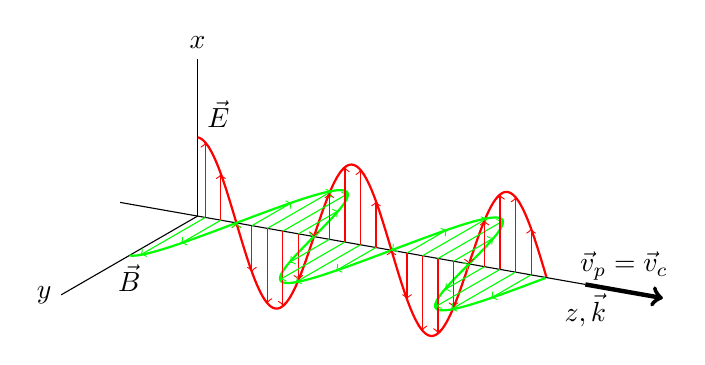
\begin{tikzpicture}[x={(-10:1cm)},y={(90:1cm)},z={(210:1cm)}]
    % Axes
    \draw (-1,0,0) -- (5,0,0) node[below] {$z, \vec{k}$};
    \draw (0,0,0) -- (0,2,0) node[above] {$x$};
    \draw (0,0,0) -- (0,0,2) node[left] {$y$};
    % Propagation
    \draw[->,ultra thick] (5,0,0) -- node[above] {$\vec{v}_p=\vec{v}_c$} (6,0,0);
    % Waves
    \draw[red,thick] plot[domain=0:4.5,samples=200] (\x,{cos(deg(pi*\x))},0);
    \draw[green,thick] plot[domain=0:4.5,samples=200] (\x,0,{cos(deg(pi*\x))});
    % Arrows
    \foreach \x in {0.1,0.3,...,4.4} {
      \draw[->,red] (\x,0,0) -- (\x,{cos(deg(pi*\x))},0);
      \draw[->,green] (\x,0,0) -- (\x,0,{cos(deg(pi*\x))});
    }
    % Labels
    \node[above right] at (0,1,0) {$\vec{E}$};
    \node[below] at (0,0,1) {$\vec{B}$};
  \end{tikzpicture}

  \begin{minipage}{.5\linewidth}
    \[
      v_p = \frac{\omega}{k} = \frac{|\vec{E}|}{|\vec{B}|} \stackrel{\text{hier}}{=} v_c
    \]
    \begin{tabular}{r@{${}={}$}p{.8\linewidth}}
      $E$ & Amplitude des elektrischen Feldes \\
      $B$ & Amplitude der Magnetflussdichte \\
      $v_p$ & Phasengeschwindigkeit \\
      $v_c$ & Lichtgeschwindigkeit im Medium\\
      $c$ &    \raggedright   Vakuum Lichtgeschwindigkeit $= \SI{299792458}{\metre\per\second}$
    \end{tabular}
  \end{minipage}%
  \begin{minipage}{.5\linewidth}
    \[
      v_c = \frac{1}{\sqrt{\mu \varepsilon}} =\frac{c}{\sqrt{\mu_r \varepsilon_r}} = \frac{c}{n} 
    \]
    \begin{tabular}{r@{${}={}$}p{.8\linewidth}}
      $\mu_0$ & magnetische Permitivität des Vakuums $= \SI{4\pi e-7}{\henry\per\metre}$ \\
      $\varepsilon_0$ &\raggedright  elektrische Permeabilität des Vakuums $= \nicefrac{1}{\mu_0 c^2}\approx \SI{8,85e-12}{\ampere\second\per(\volt\metre)}$ 
    \end{tabular}
  \end{minipage}
\end{center}
\end{frame}


\input{finalframe.inc}
   
\end{document}